\section{melcomp\_9 / ICVSfigs.m}

In melcomp\_9 several major things were introduced:

\begin{enumerate}
    \item A more extensive framework of testing a melanopic correction against other colour constancy algorithms was introduced, following the framework of \citet{barnard_comparison_2002} (later used by \citet{hordley_reevaluation_2006} and \citet{gijsenij_computational_2011}) A \gls{GW}, a \gls{BiW}, and a \gls{DN} algorithm were used as benchmarks.
    \item K-means clustering was introduced as an objective measure with which to test the requirement that clusters should be separable, which in turn relies on their tightness of clustering and the distinctness of neighbouring clusters. A k-means algorithm was passed all points with the group labels occluded, with the results being compared to the veridical groupings. An algorithm that transformed the points such that all could be categorised by group would get a perfect score of 1, whereas a hypothetical algorithm which returned the points such that none were matched to the correct group would score 0 (this is not practically possible and there will be a chance floor).
    \item The issue in melcomp\_2 whereby the transform was optimised to minimise the variance of the entire set rather than the variance within each surface-group was corrected.
    \item An additional test, whereby surfaces were randomly removed from a selection was introduced, in order to better parallel the unpredictability of surfaces in natural scenes.
\end{enumerate}

There were several important findings:

\begin{enumerate}
    \item When all surfaces are shown every time, the \gls{GW} and \gls{BiW} algorithms slightly outperform a melanopic transform.
    \item As soon as surfaces start to be randomly removed, performance of \gls{GW} and \gls{BiW} algorithms dropped sharply, whereas the melanopic transform was unaffected. \emph{Figure \ref{fig:4asum}}
    \item Similar peaks of optimality are found as were found previously (around the peak of melanopsin sensitivity and around the peak of the L-cones) but this time with the melanopsin area being `more optimal'.
\end{enumerate}

\begin{figure}[htbp]
 %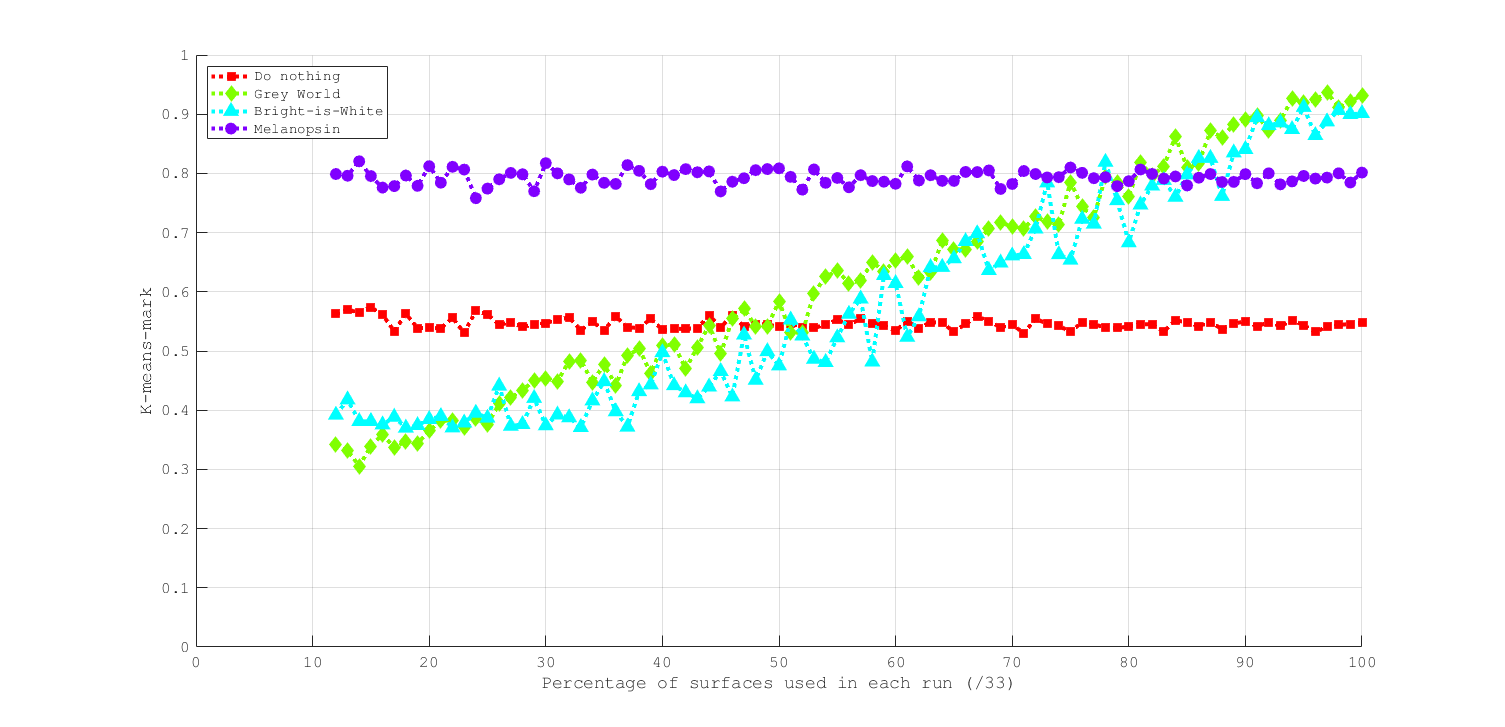
\includegraphics[max width=\textwidth]{figs/comp/melcomp_9/4a_summary.png}
 \caption{The performance of the various algorithms as a function of the available surfaces under any one simulation.}
 \label{fig:4asum}
\end{figure} 

\begin{figure}[htbp]
 %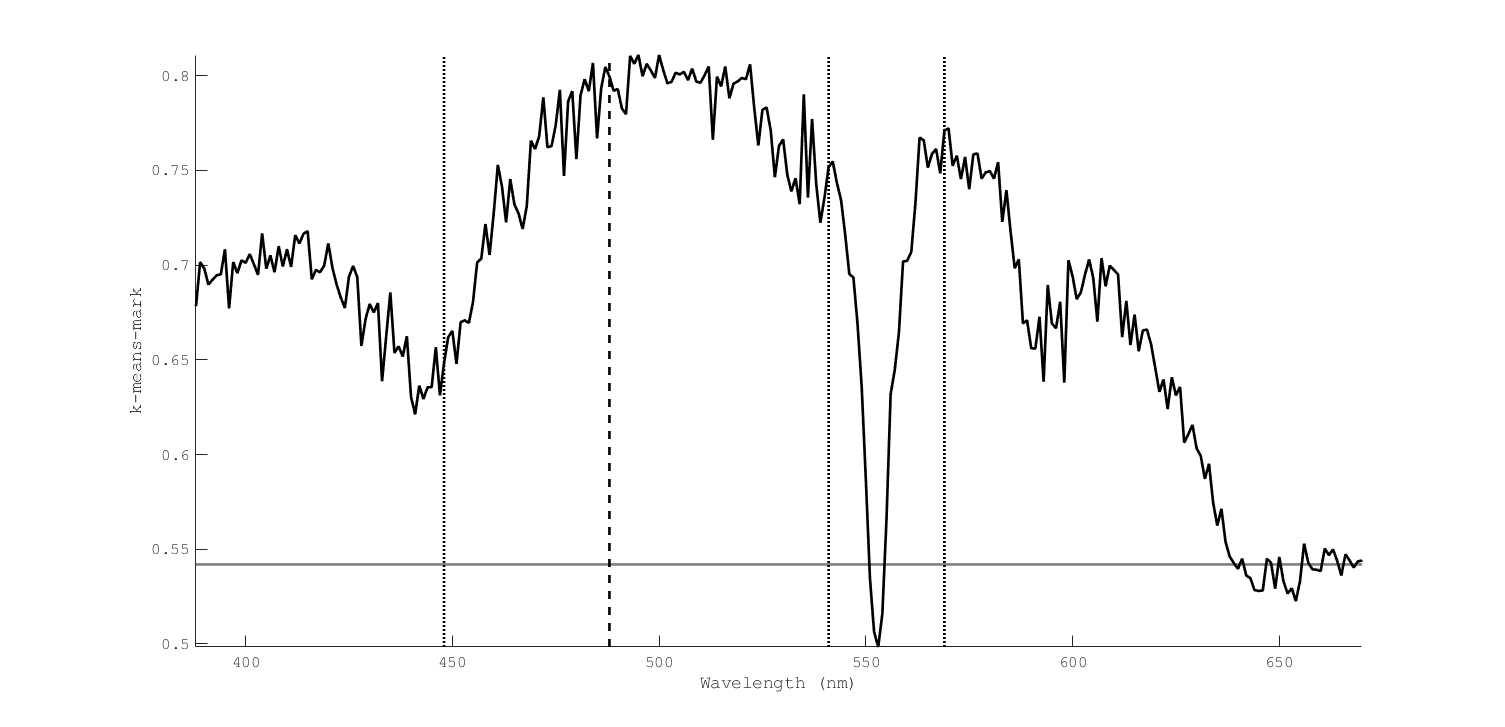
\includegraphics[max width=\textwidth]{figs/comp/melcomp_9/5a_diffMel.png.png}
 \caption{Testing the effect of shifting the melanopsin sensitivity up and down the spectrum.}
 \label{fig:9opt}
\end{figure} 

The work was presented at this stage at ICVS 2019 as an oral presentation.